\documentclass{exam}
\usepackage[utf8]{inputenc}
\usepackage{lmodern}
\usepackage{microtype}

% \usepackage[parfill]{parskip}
\usepackage[dvipsnames]{xcolor}
\usepackage{amsmath}
\usepackage{amsfonts}
\usepackage{amsthm}
\usepackage{siunitx}
\DeclareSIUnit\year{yr}
\DeclareSIUnit\foot{ft}
\DeclareSIUnit\litre{\liter}

\usepackage{skull}

\usepackage{pgfplots}
\usepgfplotslibrary{polar}
\pgfplotsset{compat=1.11}
\usepgfplotslibrary{statistics}
\usepackage{graphicx}
\usepackage{sidecap}
\sidecaptionvpos{figure}{c}
\usepackage{float}
\usepackage{gensymb}
\usepackage{tkz-euclide}
\usetkzobj{all}
\usepackage{commath}
\usepackage{hyperref}
\usepackage{enumitem}
\usepackage{wasysym}
\usepackage{multicol}
\usepackage{mathtools}
\usepackage{tcolorbox}
\usepackage{tabularx}
\usepackage[version=4]{mhchem}
\usepackage{changepage}
\usepackage{listings}
\lstset{basicstyle=\ttfamily\linespread{0.8}\small}

\renewcommand*{\thefootnote}{\fnsymbol{footnote}}

\newtheorem*{thm}{Theorem}
\newtheorem*{iden}{Identity}
\newtheorem*{lemma}{Lemma}
\newtheorem{obs}{Observation}
\theoremstyle{definition}
\newtheorem*{defn}{Definition}
\newtheorem*{ex}{Example}
\newtheorem{con}{Construction}
\newtheorem*{alg}{Algorithm}

\newtheoremstyle{break}
  {\topsep}{\topsep}%
  {\itshape}{}%
  {\bfseries}{}%
  {\newline}{}%
\theoremstyle{break}
\newtheorem*{bthm}{Theorem}

% russian integral
\usepackage{scalerel}
\DeclareMathOperator*{\rint}{\scalerel*{\rotatebox{17}{$\!\int\!$}}{\int}}

% \DeclareMathOperator*{\rint}{\int}

\pgfplotsset{vasymptote/.style={
    before end axis/.append code={
        \draw[densely dashed] ({rel axis cs:0,0} -| {axis cs:#1,0})
        -- ({rel axis cs:0,1} -| {axis cs:#1,0});
    }
}}

% \pointsinrightmargin
\boxedpoints
\pointname{}

\newcommand{\questioA}{\question[\texttt{\textbf{\color{Cerulean} A}}]}
\newcommand{\questioM}{\question[\texttt{\textbf{\color{PineGreen} M}}]}
\newcommand{\questioE}{\question[\texttt{\textbf{\color{WildStrawberry} E}}]}
\newcommand{\questioS}{\question[\texttt{\textbf{\color{Goldenrod} S}}]}
\newcommand{\questioO}{\question[\texttt{\textbf{\color{BurntOrange} O}}]}

\newcommand{\parA}{\part[\texttt{\textbf{\color{Cerulean} A}}]}
\newcommand{\parM}{\part[\texttt{\textbf{\color{PineGreen} M}}]}
\newcommand{\parE}{\part[\texttt{\textbf{\color{WildStrawberry} E}}]}
\newcommand{\parS}{\part[\texttt{\textbf{\color{Goldenrod} S}}]}
\newcommand{\parO}{\part[\texttt{\textbf{\color{BurntOrange} O}}]}

\newcommand{\subparA}{\subpart[\texttt{\textbf{\color{Cerulean} A}}]}
\newcommand{\subparM}{\subpart[\texttt{\textbf{\color{PineGreen} M}}]}
\newcommand{\subparE}{\subpart[\texttt{\textbf{\color{WildStrawberry} E}}]}
\newcommand{\subparS}{\subpart[\texttt{\textbf{\color{Goldenrod} S}}]}
\newcommand{\subparO}{\subpart[\texttt{\textbf{\color{BurntOrange} O}}]}

\newcommand{\mainHeader}[2]{\section*{NCEA Level 2 Mathematics\\#1. #2}}
\newcommand{\mainHeaderHw}[2]{\section*{NCEA Level 2 Mathematics (Homework)\\#1. #2}}
\newcommand{\seealso}[1]{\begin{center}\emph{See also #1.}\end{center}}
\newcommand{\drills}[1]{\begin{center}\emph{Drill problems: #1.}\end{center}}
\newcommand{\basedon}[1]{\begin{center}\emph{Notes largely based on #1.}\end{center}}

\begin{document}

\mainHeaderIntg{24}{Kinematics}
Calculus was independently developed by Sir Isaac Newton to describe mechanical motion in physics. This use is known as \textit{kinematics} (from
the Greek \textit{kinein}, `to move'). Suppose a particle moves from position $ x_0 $ to position $ x_1 $ over a time $ \Delta t $. We call the ratio
\begin{displaymath}
  \frac{x_1 - x_0}{\Delta t}
\end{displaymath}
the \textit{average velocity} of the particle; if we let $ x_1 \to x_2 $ (or let $ t \to 0 $), we obtain the derivative $ \od{x}{t} = v $, the
\textit{instantaneous velocity} of the particle at the point $ x $ (usually just abbreviated to velocity).

Similarly, the rate of change of velocity is called \textit{acceleration}. We have $ a = \od{v}{t} = \od[2]{x}{t} $. (Out of interest, the third
derivative of displacement is known as \textit{jerk}, and the fourth is \textit{jounce}.)

Now, suppose we know the velocity of a particle at each instant over a given time interval. Suppose we split the interval up into small intervals,
each of length $ \Delta t $. Then the total distance travelled is approximated by $ \sum v \Delta t $, where the sum is taken for each small interval.
If we make the intervals smaller, then clearly our approximation becomes better; and to obtain the true answer, we need only take an integral.

\begin{center}
  \def\arraystretch{1.5}
  \begin{tabular}{|rcc|}\hline
    \textbf{Displacement}, $ s $ && $\rint_{t_0}^{t_1} v \dif{t} $\\
    \textbf{Velocity}, $ v $ & $ \od{s}{t} $ & $ \rint_{t_0}^{t_1} a \dif{t} $\\
    \textbf{Acceleration}, $ a $ & $ \od{v}{t} $ &\\\hline
  \end{tabular}
\end{center}

We can prove the following \textit{kinematic equations} if acceleration is kept constant over a time period $ \Delta t $. These equations
should be familar to all of those that took level 2 physics, and they are derived by finding areas underneath a velocity-time graph: in
short, via calculus.

\begin{align*}
  v_f &= v_i + a \Delta t\\
  s &= v_i \Delta t + \frac{1}{2} a {\Delta t}^2\\
  v_f^2 &= v_i^2 + 2a s\\
  s &= \frac{v_f + v_i}{2} \Delta t
\end{align*}

\subsection*{Questions}
All distances are given in \si{\metre}, and all times in \si{\second}, unless otherwise stated.
\begin{questions}
  \questioA A particle moves from $ x = \SI{2}{\metre} $ to $ x = \SI{3}{\metre} $ over \SI{3}{\second}. What is its average velocity over that time?
  \questioM Derive the kinematic equations, by considering the integrals of a velocity function $ v(t) $ with constant derivative $ a $.
  \questioA A particle moves from $ (3,4) $ to $ (12,-3) $ over a time \SI{10}{\second}. If the displacements are measured in metres, what is the magnitude of
            its average velocity during that period?
  \questioA An object $ A $ has a positive acceleration $ a $, and a second object $ B $ has a negative acceleration $ -a $. Both are moving in the
            same direction. Which of the following is \textbf{not} true?
    \begin{parts}
      \part Object $ B $ is slowing down compared to object $ A $.
      \part Object $ B $ has a lower velocity than object $ A $.
      \part At some point, object $ B $ will reach a velocity of zero and then start moving in the opposite direction.
      \part If object $ B $ is behind object $ A $, the two will never cross paths.
    \end{parts}
  \questioA Suppose a particle has a velocity of $ \SI{34}{\metre\per\second} $. How long does it take for the particle to travel \SI{150}{\metre}?
  \question The velocity $ v $ of an object $ t $ seconds after it moves from the origin is given by
            \begin{displaymath}
              v(t) = 3t^2 - 6t - 24.
            \end{displaymath}
    \begin{parts}
      \parA Write down the formula for the acceleration of the particle after $ t $ seconds.
      \parA Work out the initial velocity and acceleration.
      \parA When is the object at rest momentarily?
      \parM When did the object return to the origin?
      \parE What was the total distance travelled by the object before it returned to the origin?
    \end{parts}
  \questioA A well-wrapped food parcel is dropped from an aeroplane flying at a height of \SI{500}{\metre}
            above the ground. The constant acceleration due to gravity is \SI{-9.81}{\metre\per\second\squared}. Air resistance
            is negligible.
    \begin{parts}
      \part How long does it take for the food parcel to hit the ground?
      \part How fast is the food parcel moving when it hits the ground?
    \end{parts}
  \questioA A racing car travelling at \SI{210}{\kilo\metre\per\hour} skids for a distance of \SI{150}{\metre}
            after its brakes are applied. The brakes provide a constant deceleration.
    \begin{parts}
      \part What is the deceleration in \si{\metre\per\second\squared}?
      \part How long does it take for the car to stop?
    \end{parts}
  \questioM The following is a graph of the instantaneous velocity of an object moving in one dimension over time.
            \begin{center}
              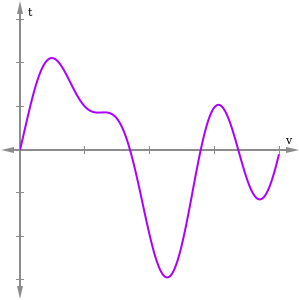
\includegraphics[width=0.3\linewidth]{velocity2}
            \end{center}
    \begin{parts}
      \part Draw the acceleration of the object over time.
      \part Draw the position of the object over time, if it was originally located at $ x = 0 $.
    \end{parts}
  \questioE The displacement of an object moving in a straight line on either side of a fixed origin is given by
            \begin{displaymath}
              s(t) = 2t^3 - 12t^2 + 18t + 3.
            \end{displaymath}
    \begin{parts}
      \part Find the minimum velocity of the object. Carefully prove that you have found a minimum.
      \part What is the distance between the origin and the object when its velocity is at a minimum?
    \end{parts}
  \questioM The velocity of an Olympic sprinter is modelled by
            \begin{displaymath}
              v_x = a(1 - e^{-bt}),
            \end{displaymath}
            where $ a = \SI{11.81}{\metre\per\second} $ and $ b = \SI{0.6887}{\per\second} $. Find an expression for the
            distance travelled after time $ t $.
  \questioM The acceleration of a rocket propelled washing machine is given by $ \od{v}{t} = 9t^3 - t^4 + t^{-3/2} $, where $ 0 \leq t \leq 10 $. Find
            the distance which it has travelled after 10 seconds if its initial velocity (at $ t = 0 $) was \SI{90}{\metre\per\second}.
\end{questions}
\end{document}
